\documentclass[../main.tex]{subfiles}
\graphicspath{{\subfix{../images/}}}
\begin{document}

Consider this other portion of $W^{(out)}$:

%Portion of the network
\begin{center}
    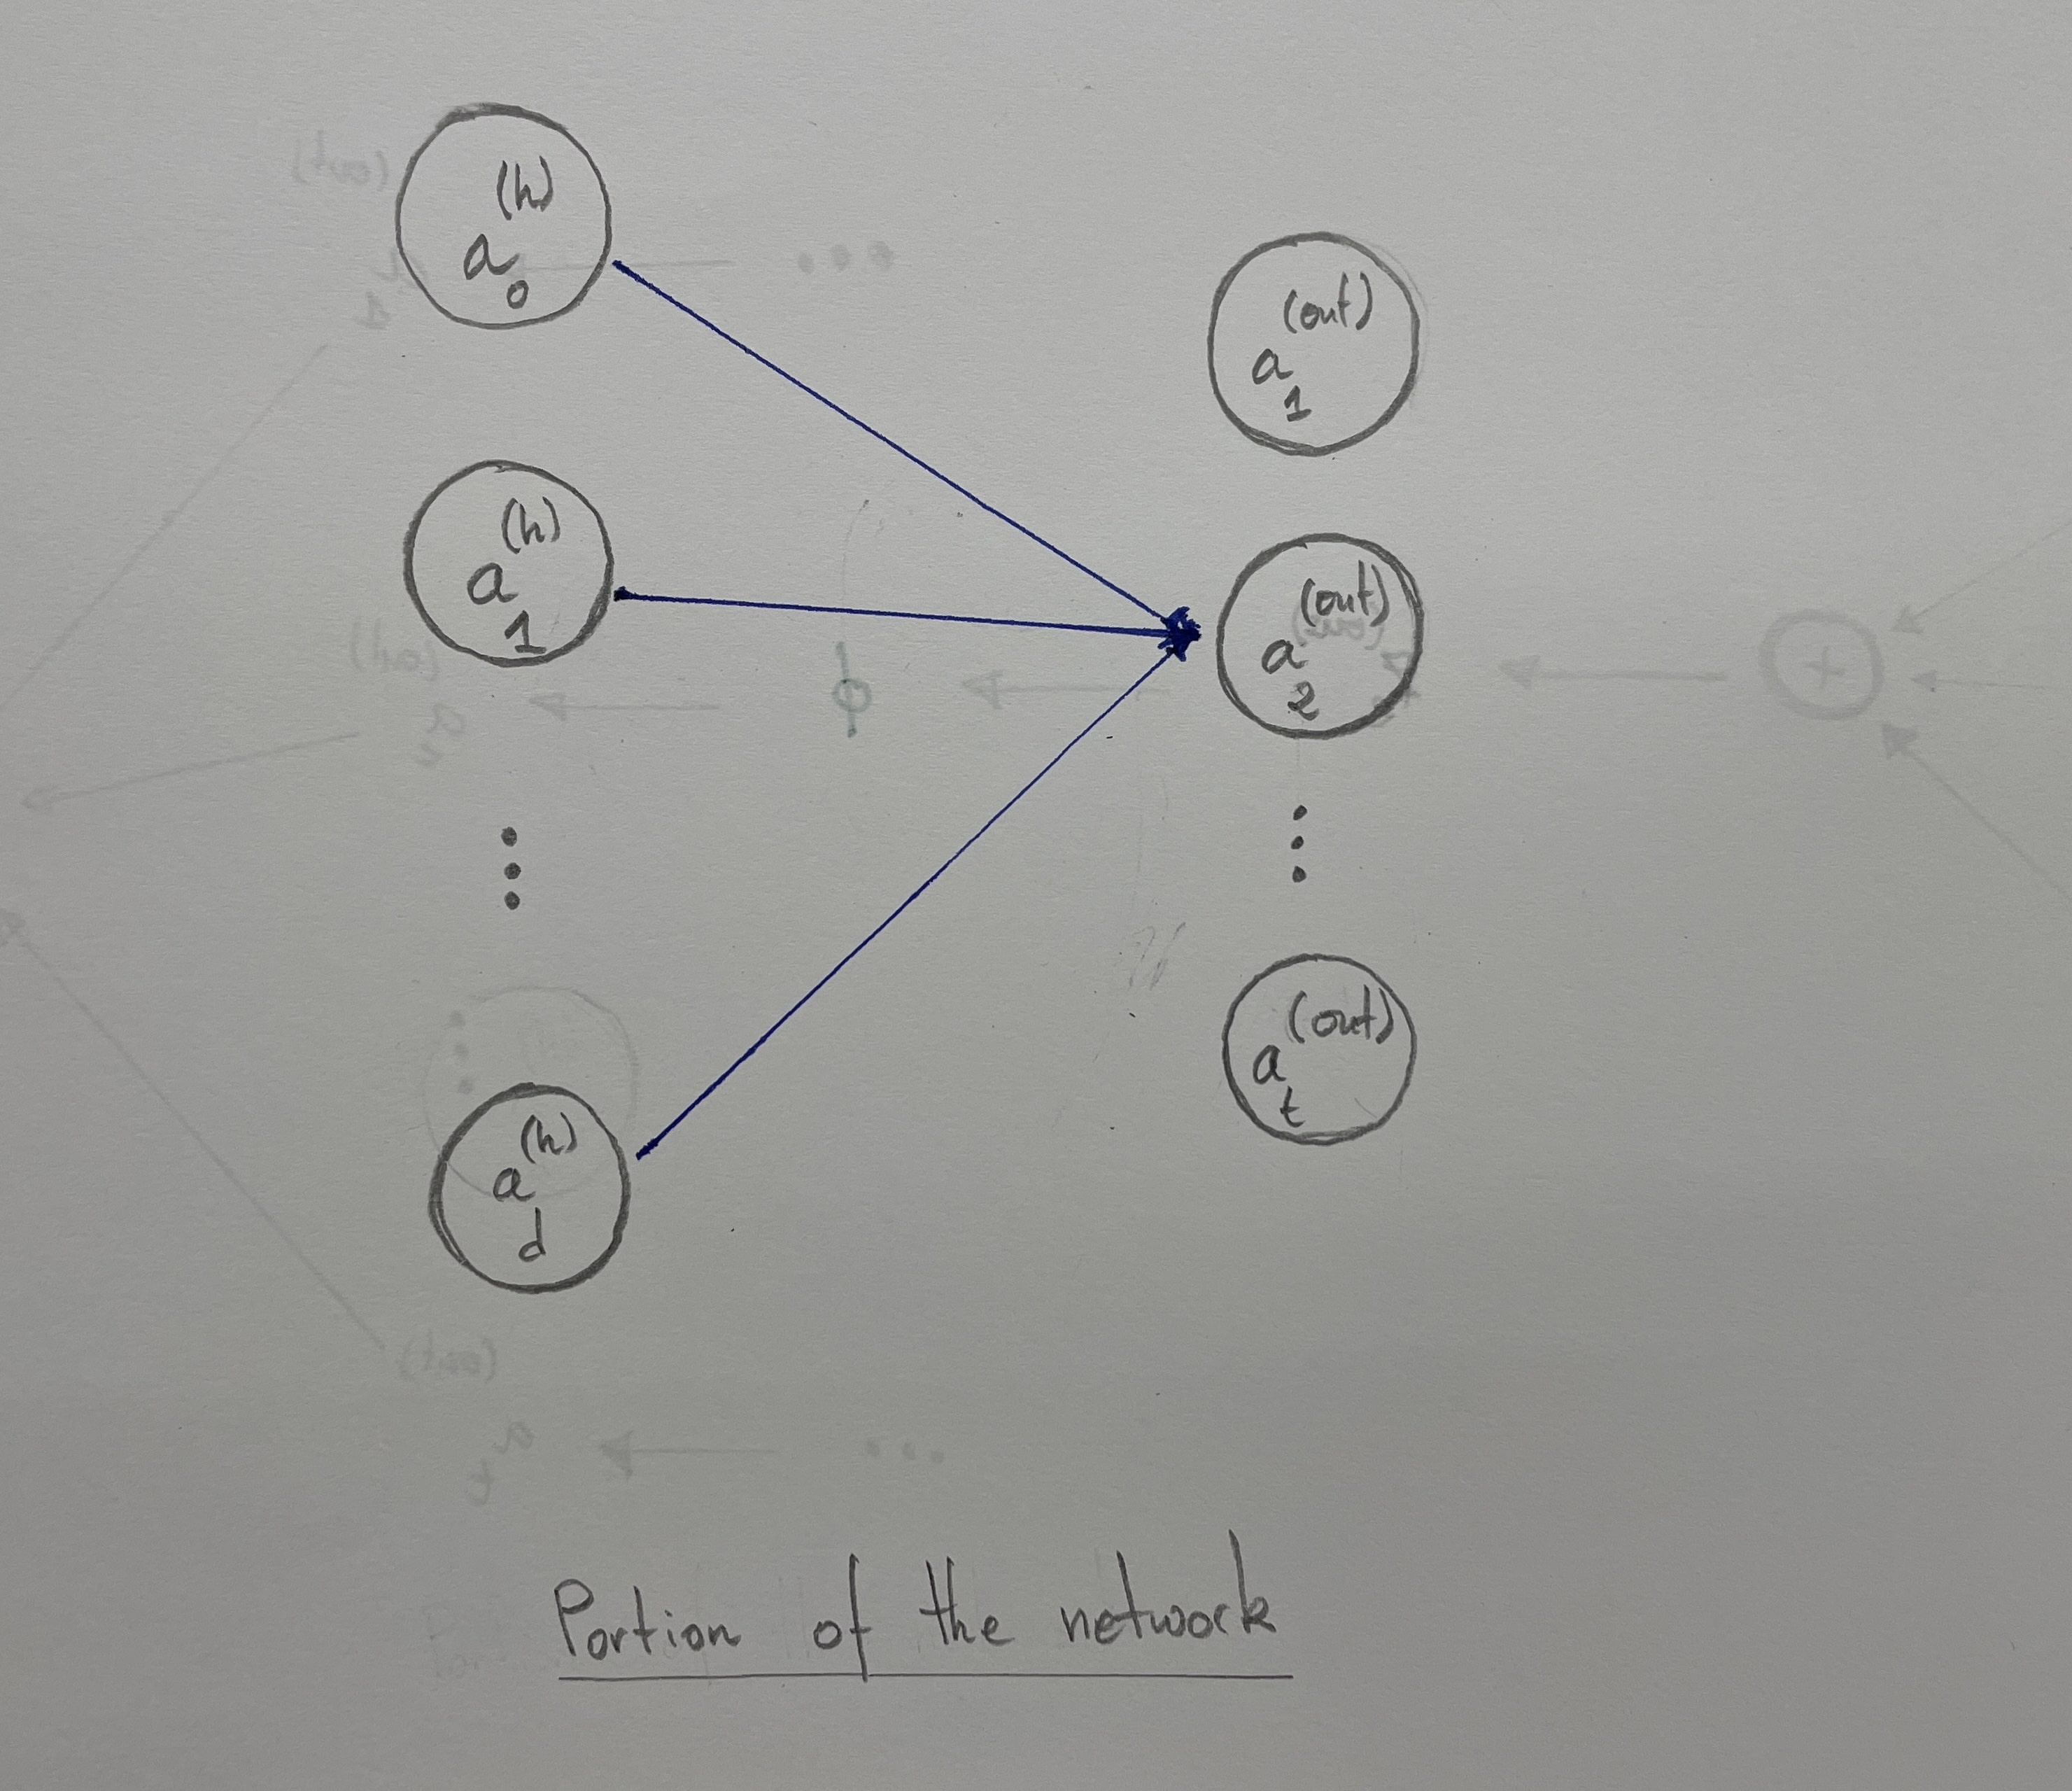
\includegraphics[width = 13cm, height = 12cm]{7.jpg}
\end{center}

\vspace{5mm} %5mm vertical space

The connections $w_{0,2}^{(out)}$, $w_{1,2}^{(out)}$, ..., $w_{d,2}^{(out)}$
are highlighted in blue. Again, let's look at them in detail... just
like we did in the previous section.

\vspace{5mm} %5mm vertical space

%Portion of the network picture
\begin{center}
    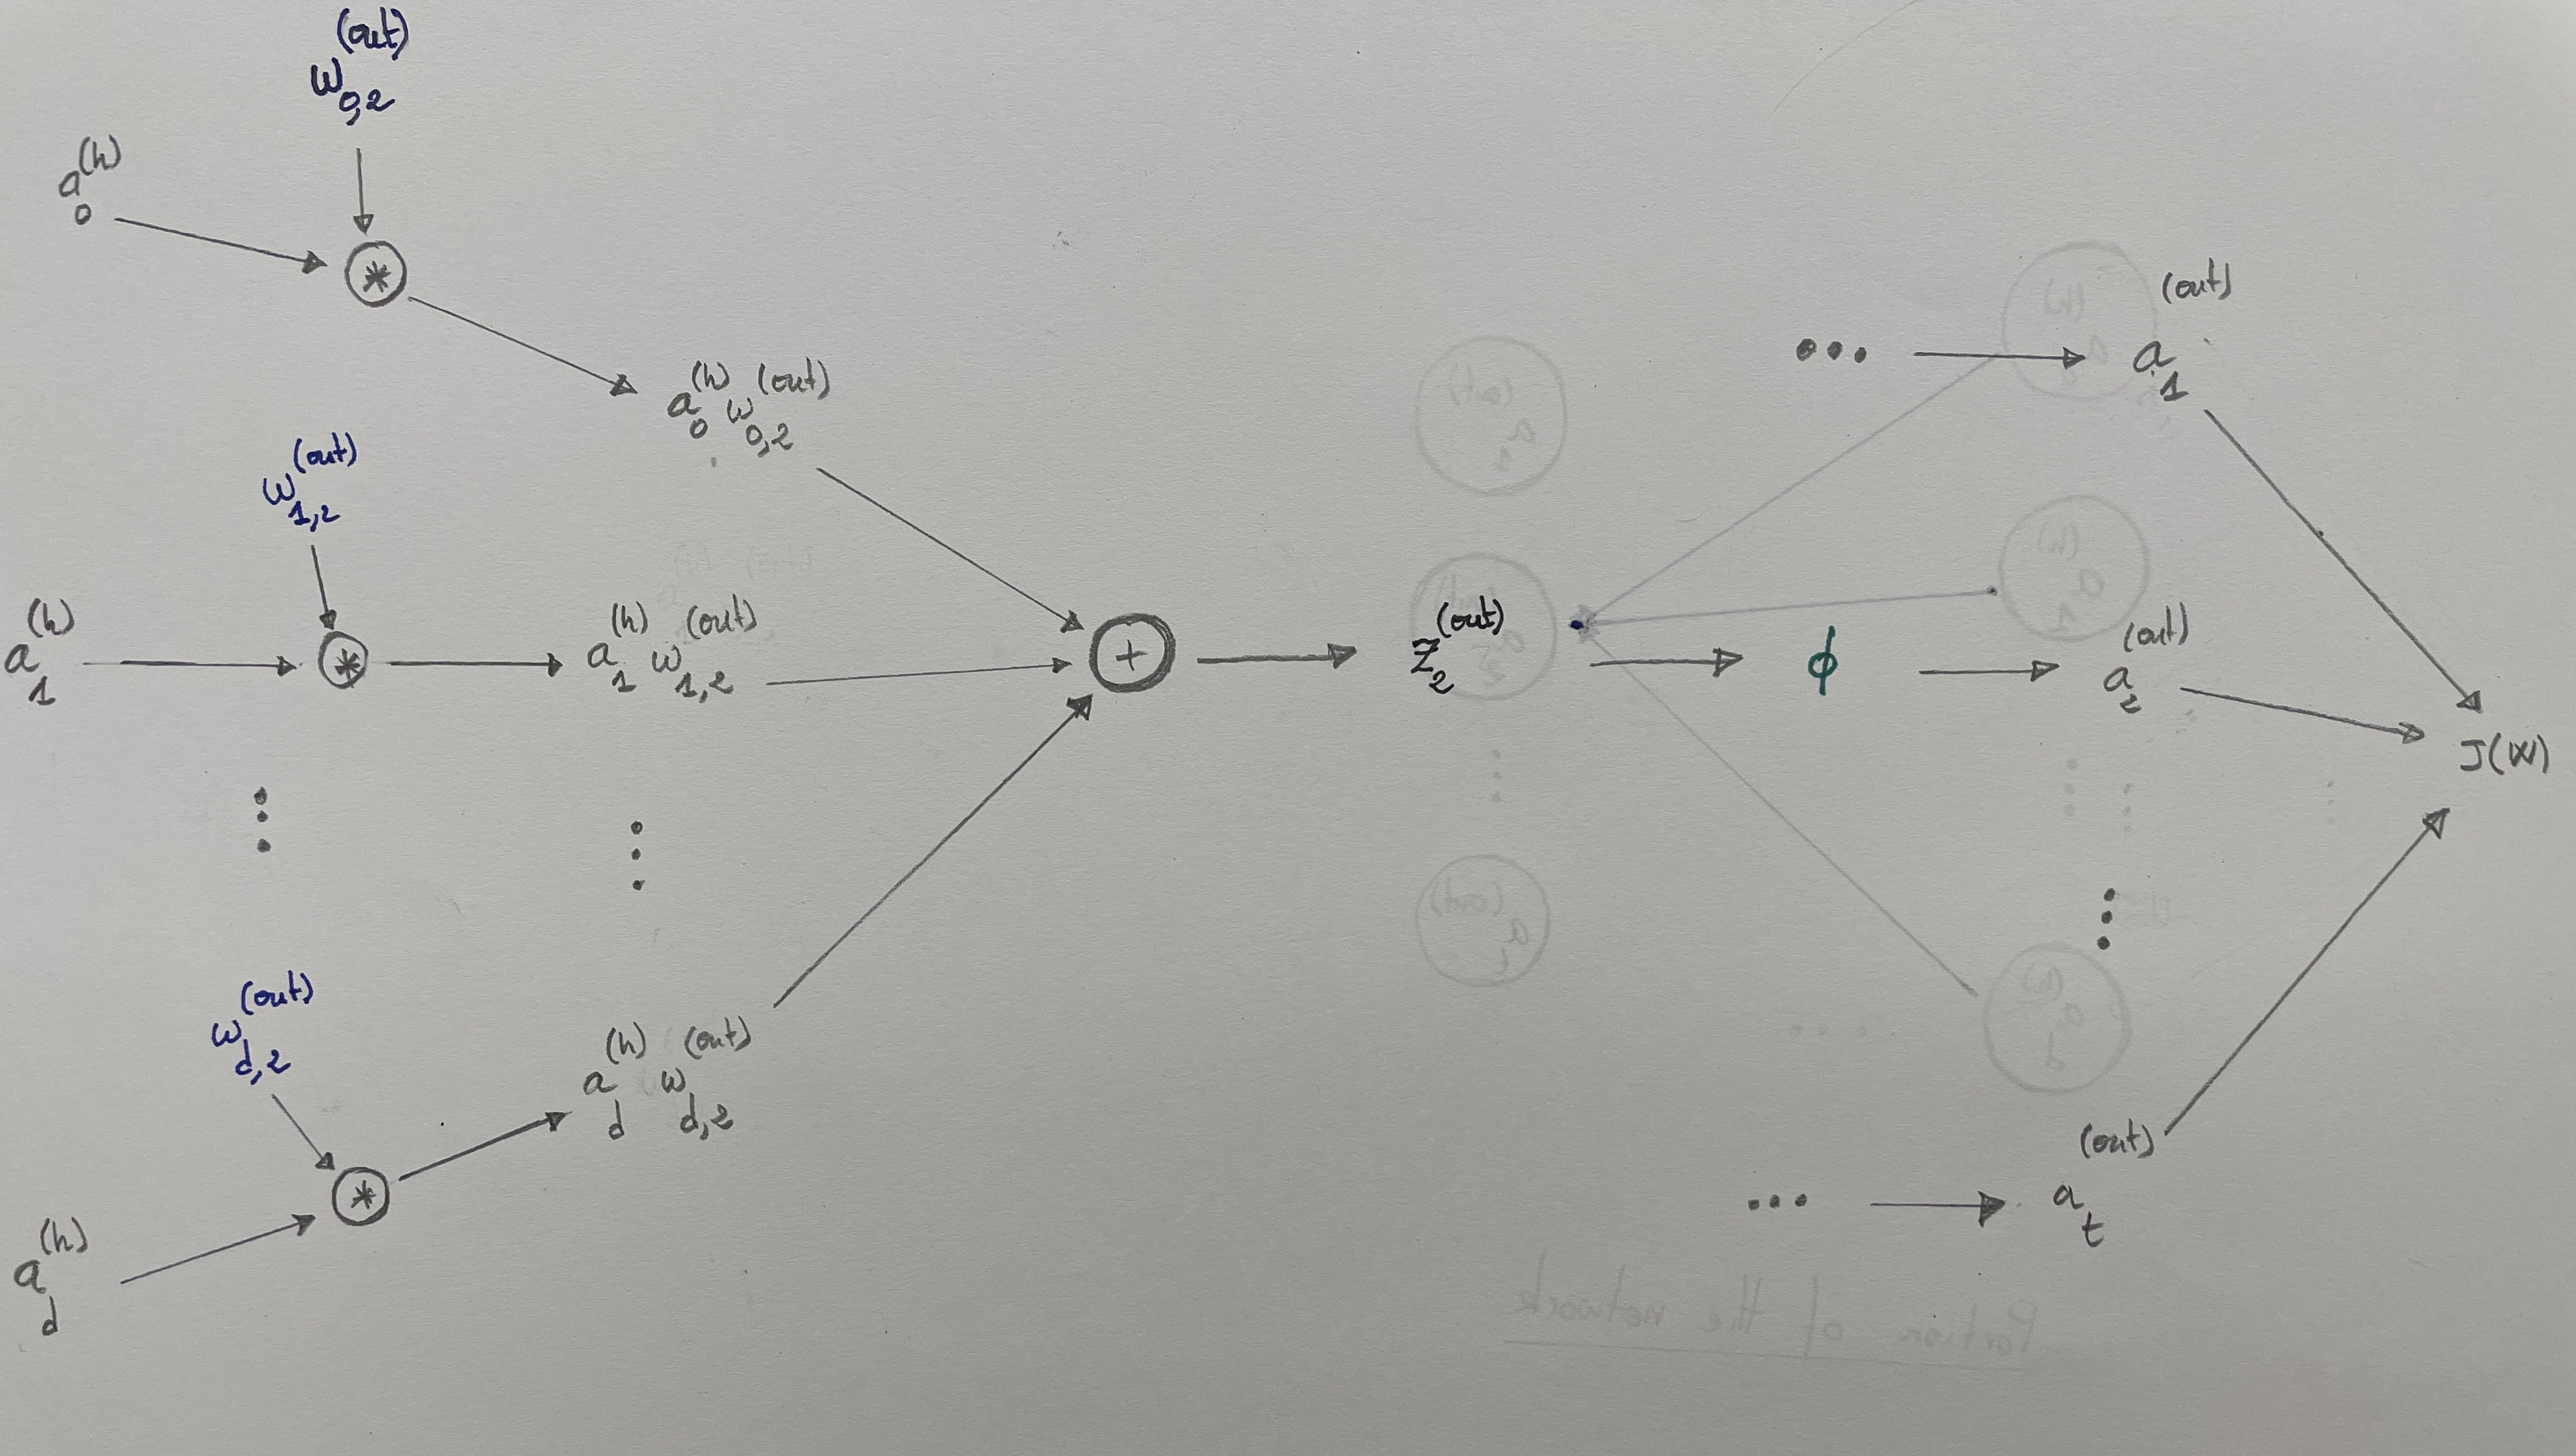
\includegraphics[width = 14cm, height = 9cm]{8.jpg}
\end{center}

\vspace{5mm} %5mm vertical space

Let's compute the gradients, starting with the loss value $J(W)$.
As you read, notice how similar the result we are about to find are to the
ones we previously found.

\[\frac{\partial J(W)}{\partial J(W)} = 1 \]

\vspace{5mm} %5mm vertical space

I continue with $a_{2}^{(out)}$

\[
    \frac{\partial J(W)}{\partial a_{2}^{(out)}} =
    \frac{a_{2}^{(out)} - y_{2}}{a_{2}^{(out)}(1 - a_{2}^{(out)})}
\]

\vspace{5mm} %5mm vertical space

Moving on with $z_{2}^{(out)}$

\[
    \frac{\partial J(W)}{\partial z_{2}^{(out)}} =
    \frac{\partial a_{2}^{(out)}}{\partial z_{2}^{(out)}} \times
    \frac{\partial J(W)}{\partial a_{2}^{(out)}} =
    a_{2}^{(out)}(1 - a_{2}^{(out)}) \bullet \frac{\partial J(W)}{\partial a_{2}^{(out)}} =
    a_{2}^{(out)} - y_2
\]

\vspace{5mm} %5mm vertical space

Let's continue with: $a_0^{(h)}w_{0,2}^{(out)}$, $a_1^{(h)}w_{1,2}^{(out)}$, ..., $a_d^{(h)}w_{d,2}^{(out)}$


\[
    \frac{\partial J(W)}{\partial a_0^{(h)}w_{0,2}^{(out)}} =
    \frac{\partial J(W)}{\partial a_1^{(h)}w_{1,2}^{(out)}} =
    \dots =
    \frac{\partial J(W)}{\partial a_d^{(h)}w_{d,2}^{(out)}} = 
    a_{2}^{(out)} - y_2
\]

\vspace{5mm} %5mm vertical space

Conveniently, they also have the same gradients.

\vspace{5mm} %5mm vertical space

We can now determine the gradients of $w_{0,2}^{(out)}$, $w_{1,2}^{(out)}$, ..., $w_{d,2}^{(out)}$.
Here again, I will ignore the bias weight $w_{0,2}^{(out)}$, but will come to it later. I promise.

\[
    \frac{\partial J(W)}{\partial w_{1,2}^{(out)}} =
    \frac{\partial a_1^{(h)}w_{1,2}^{(out)}}{\partial w_{1,2}^{(out)}} \times
    \frac{\partial J(W)}{\partial a_1^{(h)}w_{1,2}^{(out)}}  =
    a_1^{(h)}(a_{2}^{(out)} - y_{2})
\]

\[ \vdots \]

\[
    \frac{\partial J(W)}{\partial w_{d,2}^{(out)}} =
    \frac{\partial a_d^{(h)}w_{d,2}^{(out)}}{\partial w_{d,2}^{(out)}} \times
    \frac{\partial J(W)}{\partial a_d^{(h)}w_{d,2}^{(out)}}  =
    a_d^{(h)}(a_{2}^{(out)} - y_{2})
\]

\vspace{1cm} %1cm vertical space

Please notice once again, how $a_{2}^{(out)} - y_{2}$ repeats in the results
we found. Let's call it $\delta_2^{(out)}$.

\vspace{1cm} %1cm vertical space

We now know the gradients of $w_{0,2}^{(out)}$, $w_{1,2}^{(out)}$, ..., $w_{d,2}^{(out)}$.
Let's move our attention to another part of the network.

\end{document}